\documentclass[t,aspectratio=169]{beamer}

\usepackage{soul}
\usepackage{multicol}
\usepackage[utf8]{inputenc}

% ----------------------------------------------------------------------------------------------------------------------------------------

\title{
\includegraphics[width=45pt]{oepecsetlogo.png}\\(KTXFI2EBNF) Physics II. Lecture}

% \subtitle{1-4. lecture}

\author{Dr.~Gábor FACSKÓ, PhD\\\tiny Assistant Professor / Senior Research Fellow\\\textit{facsko.gabor@uni-obuda.hu}}

\institute{\Tiny Óbuda University, Faculty of Electrical Engineering, 1084 Budapest, Tavaszmező u. 17.\\Wigner Research Centre for Physics, Department of Space Physics and Space Technology, 1121 Budapest, Konkoly-Thege Miklós út 29–33.\\ \url{https://wigner.hu/~facsko.gabor}}

\date{October 13,~2025}

\logo{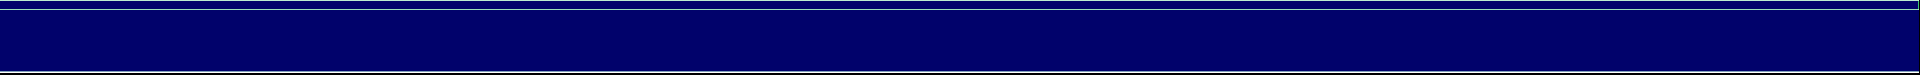
\includegraphics[height=0.9 true cm]{kekcsik.png}}

% ----------------------------------------------------------------------------------------------------------------------------------------

\begin{document}

\frame{\titlepage}

% ----------------------------------------------------------------------------------------------------------------------------------------

\begin{frame}[fragile,squeeze,allowframebreaks]
\frametitle{Status Report}
\begin{itemize}
\setlength{\parskip}{0pt}
\setlength{\itemsep}{0pt}
\item No communication with Mr.~Szilárd~ZSÓKA. :(
\item You need to do your homework and take a test – no practice.
\item How many tests should you take?
\item I give my lectures and do the exercises with you. 
\end{itemize}
\end{frame}

% ----------------------------------------------------------------------------------------------------------------------------------------

\begin{frame}[fragile,squeeze,allowframebreaks]
\frametitle{Where are we?}
\begin{itemize}
\setlength{\parskip}{0pt}
\setlength{\itemsep}{0pt}
\item \st{Motion of charged particles in electromagnetic fields.}
\item \st{Elements of quantum mechanics. Heisenberg's uncertainty principle. The stationary Schrödinger equation and its applications.}
\item \st{Limits of the classical conceptual framework. Thermal radiation. Photoelectric effect. Compton effect. The dual nature of electromagnetic radiation. The dual nature of particles.}
\item \textbf{Moving reference frames. Inertial forces in accelerating reference frames. Elements of special relativity. Dirac-equation, antimatter.}
\item \textit{The classical theory of atomic structure (Rutherford, Franck-Hertz experiment, Bohr model, quantum numbers, Pauli exclusion principle).}
\item Physics of condensed matter. Metallic bonding. Electrical conduction in metals based on the free electron model and the wave model. Hall effect. Band theory of solids.
\pagebreak
\item Semiconductors. Elements of Fermi-Dirac statistics. Thermoelectric phenomena. Magnetic properties.  
\item Ferroelectricity. Piezoelectricity and electrostriction. Liquid crystals. Superconductivity.
\item Luminescence. Lasers. Basic knowledge of nuclear physics. Basic knowledge of particle physics.
\end{itemize}
\end{frame}

% ----------------------------------------------------------------------------------------------------------------------------------------

\begin{frame}[fragile,squeeze,allowframebreaks]
  \frametitle{Elements of the Special Relativity Theory -- Clarification}
\vskip -10 pt
\begin{itemize}
\setlength{\parskip}{0pt}
\setlength{\itemsep}{0pt}
\item Special Relativity Theory vs.~General Relativity Theory: both are classical theories.
\item Special Relativity Theory: reference frames moving uniformly in a straight line
\begin{itemize}
\item Lorentz, Minkowski, Einstein, and others
\item Lorentz transformation, time dilation, mass increase, addition of velocities, electrodynamics, Maxwell's equations
\item Quantum Mechanics + Special Relativity Theory = Dirac equation, positron, antimatter, Relativistic Quantum Electrodynamics, Quantum Chromodynamics, Quarks, Higgs boson
\end{itemize}
\item General Relativity Theory: any reference frame 
\begin{itemize}
\item Gravitational theory: a geometrical theory
\item Time dilation caused by gravitation (GPS!)
\item Gravitational lenses
\item Developed by Albert~Einstein (with help from his wife and a circle of mathematician friends)
\item \textbf{ASSIGNMENT: Watch (again) the \textit{Interstellar} movie.}
\end{itemize}
\end{itemize}
\pagebreak
\begin{center}
\includegraphics[width=0.9\textwidth]{images-20251013/blackhole.png}\\ 
The spacetime is twisted, therefore, we can the accretion disc behind the black hole.
\end{center}
\pagebreak
\begin{center}
\includegraphics[width=0.65\textwidth]{images-20251013/gravitationallens.png}\\ 
The massive object bends the light curve and behaves as a lens. 
\end{center}
\end{frame}

% ----------------------------------------------------------------------------------------------------------------------------------------

\begin{frame}[fragile,squeeze,allowframebreaks]
\frametitle{Galilean Principle of Relativity, Galilean Transformations}
\begin{itemize}
\setlength{\parskip}{0pt}
\setlength{\itemsep}{0pt}
\item Description of motion in reference frames moving uniformly in a straight line
\item Reference frames performing uniform linear motion: Galilean principle of relativity
\item On a straight railway track, a passenger train is either at rest or moving with a constant (magnitude and direction) velocity. Sitting in a completely curtained passenger car, can one decide — without looking out of the windows — whether the train is at rest or in motion? Can we feel, through our body, what kind of motion state the train is in?
\medskip
\begin{center}
\includegraphics[width=0.25\textwidth]{images-20251013/bzmot.jpg}
\includegraphics[width=0.25\textwidth]{images-20251013/bzmot2.jpg}
\includegraphics[width=0.25\textwidth]{images-20251013/bzmot3.jpg}
\end{center}
\pagebreak
\item What forces act on a body resting at a point $P$ in space when observed from a uniformly moving reference frame?
\begin{center}
\includegraphics[width=0.5\textwidth]{images-20251013/galilei.png}
\end{center}
K: reference frame at rest\\
K': reference frame moving with velocity $\mathbf{v_{0}}$ relative to K
\pagebreak
\item From the vector triangle OO'P: $$\mathbf{r_{o}}+\mathbf{r'}=\mathbf{r}.$$
\item Differentiating both sides with respect to time: $$\mathbf{v_{o}}+\mathbf{v'}=\mathbf{v}.$$
\item Differentiating again with respect to time: $$\mathbf{a_{o}}+\mathbf{a'}=\mathbf{a},$$ then multiplying by the mass $m$: $$m\mathbf{a'}=m\mathbf{a}.$$
  \pagebreak
\item Therefore, $$\mathbf{F'}=\mathbf{F}.$$
\item \underline{Galilean Principle of Relativity:} Reference frames that are at rest or moving uniformly and linearly relative to each other are completely equivalent with respect to mechanical phenomena. If one of them is an inertial frame, then all of them are.
\item \underline{Consequence of the Galilean Principle of Relativity:} If there exists one inertial frame, then infinitely many inertial frames exist. \\ \, \\ Newton’s First Law: There exists a reference frame in which ... This is an inertial frame. $\rightarrow$ Therefore, an inertial frame exists, and infinitely many exist.
\pagebreak
\item Galilean Transformations:
\vskip -35 pt
\begin{eqnarray*}
\mathbf{r_{o}}+\mathbf{r'}&=&\mathbf{r},\\
\mathbf{v_{o}}+\mathbf{v'}&=&\mathbf{v},\\
\mathbf{a'}&=&\mathbf{a},\\
\mathbf{t'}&=&\mathbf{t}.
\end{eqnarray*}
 \begin{center}ű
\includegraphics[width=0.5\textwidth]{images-20251013/galilei.png}
\end{center}
\pagebreak
\item What about other physical phenomena when we apply Galilean transformations to their descriptive equations? Do the equations remain equivalent or not? For example: in electromagnetism — are Maxwell’s equations invariant under Galilean transformations?
\item What about light? Does the speed of light add to the velocity of moving objects? For example: does the velocity of light emitted on a moving train add to (or subtract from) the train’s velocity?
\medskip
\item \underline{Light clock:} A light clock is a tube with a plane mirror at one end and a flashing light source installed on the tube’s central axis at the other end.\\
\begin{center}
\includegraphics[width=0.45\textwidth]{images-20251013/light_clock.png}
\end{center}
\pagebreak
\item Light Clock Experiment
\begin{center}
\includegraphics[width=0.9\textwidth]{images-20251013/light_clock_experiment.png}
\end{center}
\pagebreak
\item Light Clock Experiment - cont'd
\begin{center}
\includegraphics[width=0.9\textwidth]{images-20251013/light_clock_experiment2.png}
\end{center}
\pagebreak
\item Train Experiment
\begin{center}
\includegraphics[width=0.9\textwidth]{images-20251013/train_experiment.png}
\end{center}
\pagebreak
\item Michelson-Morley Experiment: No interference
\begin{center}
\includegraphics[width=0.9\textwidth]{images-20251013/mm_experiment.png}
\end{center}
\end{itemize}
\end{frame}

% ----------------------------------------------------------------------------------------------------------------------------------------

\begin{frame}[fragile,squeeze,allowframebreaks]
\frametitle{Lorentz Transformations}
\begin{itemize}
\setlength{\parskip}{0pt}
\setlength{\itemsep}{0pt}
\item Reference frames for Lorentz transformations
\begin{center}
\includegraphics[width=0.8\textwidth]{images-20251013/lorentz.png}
\end{center}
\pagebreak
\,  
\vskip -30 pt
\begin{columns}
  \begin{column}{0.45\textwidth}
    \begin{center}
\textbf{Lorentz Transformations}
\begin{eqnarray*}
t'&=&\frac{t-\frac{v}{c^{2}}x}{\sqrt{1-\frac{v^{2}}{c^{2}}}}\\
x'&=&\frac{x-vt}{\sqrt{1-\frac{v^{2}}{c^{2}}}}\\
y'&=&y\\
z'&=&z
\end{eqnarray*}
\end{center}
\end{column}
\begin{column}{0.45\textwidth}
\begin{center}
\textbf{Inverse Transformations}
\begin{eqnarray*}
t&=&\frac{t'+\frac{v}{c^{2}}x'}{\sqrt{1-\frac{v^{2}}{c^{2}}}}\\
x&=&\frac{x'+vt'}{\sqrt{1-\frac{v^{2}}{c^{2}}}}\\
y&=&y'\\
z&=&z'
\end{eqnarray*}
\end{center}
\end{column}
\end{columns}
\medskip
$t, t'$: time; $x, x'$, $y, y'$, $z, z'$: coordinates; $v$: velocity of the $K'$ frame; $c$: speed of light\\
$t, x, y, z$ belong to the $K$ reference frame, $t', x', y', z'$ belong to the $K'$ reference frame

\pagebreak
\item Consequences of the Lorentz transformation
\begin{itemize}
\item For $v > c$ there is no real solution (thus $v > c$ is impossible)
\item For $v \ll c$ it reduces to the previously known Galilean principle of relativity
\item Convention: if $v \le c/6$, a non-relativistic description should be used
\item The concept of simultaneity is relative
\item Length contraction (``Einstein's garage''): $$l' = l \sqrt{1-\frac{v^{2}}{c^{2}}}.$$
\item Time dilation (``Twin Paradox''): $$\Delta t=\frac{\Delta t'}{\sqrt{1-\frac{v^{2}}{c^{2}}}}.$$
\end{itemize}
\end{itemize}
\end{frame}

% ----------------------------------------------------------------------------------------------------------------------------------------

\begin{frame}%[fragile,squeeze,allowframebreaks]
\frametitle{Einstein's Postulates}
\begin{itemize}
\setlength{\parskip}{0pt}
\setlength{\itemsep}{0pt}
\item \underline{Principle of Equivalence:} All inertial reference frames are equivalent for describing any physical phenomenon.  
In other words, reference frames that are at rest or move uniformly in a straight line relative to each other are equivalent for all physical laws.
\item \underline{Principle of the Constancy of the Speed of Light:}  
The speed of light is a universal constant, independent of the motion of the source, the observer, or the reference frame.  
Its value is $c \approx 3 \cdot 10^{8}\,\mathrm{m/s}$.  
The speed of light in vacuum is the ultimate speed limit — it cannot be reached or exceeded by any object.
\item Comment: Cherenkov radiation :)
\item Applying these principles to the Michelson–Morley experiment, we obtain $t_{\parallel} \ne t_{\perp}$.  
\textit{Conclusion:} time flows at different rates.
\end{itemize}
\end{frame}

% ----------------------------------------------------------------------------------------------------------------------------------------

\begin{frame}[fragile,squeeze,allowframebreaks]
\frametitle{Relativistic Dynamics}
\begin{itemize}
\setlength{\parskip}{0pt}
\setlength{\itemsep}{0pt}
\item \underline{Relativistic mass increase:}  
$$m=\frac{m_{0}}{\sqrt{1-\frac{v^{2}}{c^{2}}}},$$  
where $m_{0}$ is the rest mass, $m$ is the relativistic mass, $c$ is the speed of light, and $v$ is the velocity.
\item \underline{Momentum:}  
$$p = m v = \frac{m_{0}v}{\sqrt{1-\frac{v^{2}}{c^{2}}}}.$$
\item \underline{Total energy:}  
$$E = W = m c^{2} = \frac{m_{0} c^{2}}{\sqrt{1-\frac{v^{2}}{c^{2}}}}.$$
\pagebreak
\item \underline{Rest energy:}  
$$E_{0} = W_{0} = m_{0}c^{2}.$$
\item \underline{Kinetic energy:}  
$$W_{\text{kin}} = W - W_{0} = m c^{2} - m_{0} c^{2} = \frac{m_{0} c^{2}}{\sqrt{1-\frac{v^{2}}{c^{2}}}} - m_{0} c^{2}.$$
\item \underline{Fundamental equation of relativistic dynamics:}  
  $$\mathbf{F} = \frac{d\left(m\mathbf{v}\right)}{dt}=\frac{dm}{dt}\mathbf{v}+m\frac{d\mathbf{v}}{dt}=\frac{dm}{dt}\mathbf{v}+m\mathbf{a}.$$
\pagebreak
\item \underline{Equivalence of mass and energy:}  Mass and energy are inseparable manifestations of matter.
\end{itemize}
\end{frame}

% ----------------------------------------------------------------------------------------------------------------------------------------

\begin{frame}[fragile,squeeze,allowframebreaks]
\frametitle{The Dirac Equation and Its Physical Meaning}
\begin{itemize}
\setlength{\parskip}{3pt}
\setlength{\itemsep}{3pt}

\item \underline{Dirac equation (in covariant form):}
$$\left( i \hbar \gamma^{\mu} \partial_{\mu} - m c \right) \psi = 0$$

\item \underline{Explanation of symbols:}
\begin{itemize}
\item $\psi$ : Dirac spinor (a four-component wave function describing spin-$\tfrac{1}{2}$ particles, e.g. electrons)
\item $m$ : rest mass of the particle
\item $c$ : speed of light in vacuum
\item $\hbar$ : reduced Planck constant ($\hbar = \frac{h}{2\pi}$)
\item $\partial_{\mu}$ : four-gradient operator  
      $$\partial_{\mu} = \left( \frac{1}{c}\frac{\partial}{\partial t}, -\nabla \right)$$
\item $\gamma^{\mu}$ : Dirac gamma matrices ($\mu = 0,1,2,3$), satisfying  
      $$  \{ \gamma^{\mu}, \gamma^{\nu} \} = 2 g^{\mu\nu} I, $$
      where $g^{\mu\nu}$ is the Minkowski metric tensor and $I$ is the identity matrix.
\end{itemize}

\item \underline{Alternative (Hamiltonian) form:}
$$ i \hbar \frac{\partial \psi}{\partial t} = \left( -i \hbar c\, \boldsymbol{\alpha} \cdot \nabla + \beta m c^{2} \right) \psi, $$
where $\boldsymbol{\alpha}$ and $\beta$ are $4\times4$ Dirac matrices defined by  
$\alpha^{i} = \gamma^{0}\gamma^{i}$ and $\beta = \gamma^{0}$.

\pagebreak

\item \underline{Physical meaning:}
\begin{itemize}
\item The Dirac equation unifies \textbf{quantum mechanics} and \textbf{special relativity}.
\item It correctly describes particles with \textbf{spin $\tfrac{1}{2}$} and predicts their intrinsic \textbf{magnetic moment}.
\item It naturally introduces the concept of \textbf{antimatter} — particles with the same mass but opposite charge (e.g. the positron).
\item The equation ensures that the probability density remains positive and conserved under Lorentz transformations.
\item At low velocities ($v \ll c$), it reduces to the Schrödinger equation, ensuring consistency with non-relativistic quantum mechanics.
\end{itemize}

\end{itemize}
\end{frame}

% ----------------------------------------------------------------------------------------------------------------------------------------

\begin{frame}[fragile,squeeze,allowframebreaks]
\frametitle{Consequences of the Dirac Equation}
\begin{itemize}
\setlength{\parskip}{4pt}
\setlength{\itemsep}{4pt}

\item \underline{Existence of spin:}
\begin{itemize}
\item The Dirac equation naturally describes particles with \textbf{intrinsic spin $\tfrac{1}{2}$}.
\item The spin is a purely quantum mechanical property with no classical analogue.
\item The spin arises from the four-component structure of the Dirac spinor.
\end{itemize}

\item \underline{Magnetic moment:}
\begin{itemize}
\item The equation predicts the correct magnetic moment of the electron:
\[
\boldsymbol{\mu} = g \frac{e \hbar}{2 m} \mathbf{S}, \quad \text{with } g = 2.
\]
\item This prediction agrees very closely with experimental data (after quantum electrodynamic corrections).
\end{itemize}
\pagebreak
\item \underline{Negative energy solutions:}
\begin{itemize}
\item The Dirac equation allows both positive and negative energy states: $$E = \pm \sqrt{p^{2} c^{2} + m^{2} c^{4}}.$$
\item Initially a theoretical puzzle, later interpreted as the existence of \textbf{antiparticles}.
\end{itemize}

\item \underline{Antimatter:}
\begin{itemize}
\item The negative-energy solutions correspond to particles with the same mass but opposite charge.
\item This led to the prediction — and later experimental discovery — of the \textbf{positron} in 1932 (by Carl~D.~Anderson).
\pagebreak
\item Annihilation
\begin{center}
\includegraphics[width=0.95\textwidth]{images-20251013/annihilation.png}
\end{center}
\end{itemize}

\pagebreak

\item \underline{Relativistic quantum field theory:}
\begin{itemize}
\item The Dirac equation laid the foundation for \textbf{Quantum Electrodynamics (QED)}.
\item It describes interactions between charged spin-$\tfrac{1}{2}$ particles and electromagnetic fields.
\item This framework explains atomic structure, scattering, and vacuum fluctuations with exceptional precision.
\end{itemize}

\item \underline{Summary:}
\begin{itemize}
\item The Dirac equation unifies:
  \begin{itemize}
    \item Quantum mechanics (wave–particle duality),
    \item Special relativity (Lorentz invariance),
    \item and Intrinsic spin (a fundamental property of matter).
  \end{itemize}
\item It remains one of the cornerstones of modern physics.
\end{itemize}

\end{itemize}
\end{frame}


% ----------------------------------------------------------------------------------------------------------------------------------------

\begin{frame}
%\frametitle{Minden jó, ha a vége jó}

\vfill
\begin{center}
\textbf{\huge The End}

\bigskip
Thank you for your attention!
\end{center}
\vfill
\end{frame}

\end{document}
